\chapter{Theoretical Framework}

Typical galaxies all around the Universe hold different structures such as stellar systems of between $ 10^{2} $ and $ 10^{6} $ stars which orbit their galactic core . We call these interesting systems star clusters and they are basically divided into two main types: Open Clusters and \textbf{Globular Clusters}. 

\section{Globular Clusters}


Globular clusters are very massive stellar systems that can contain from thousands to millions of stars in a nearly spherical distribution spread over a volume of several tens to about 200 light years in diameter. These stellar systems are composed of old stars and they do not contain gas or dust. 

The average star density in a Globular Cluster is about 0.4 stars per cubic parsec. In the dense center of the cluster, the star density can increase from 100 to 1000 per cubic parsec. However, even in the center of clusters, there is still plenty of space between the stars

A way of analysing globular clusters is to use Colour-Magnitude diagrams. A colour-magnitude diagram is a plot of the apparent magnitudes of the stars in a cluster against their colour indices. Globular clusters nearly all have very similar colour-magnitude diagrams

Globular clusters revolve about the nucleus of a galaxy on orbits of high eccentricity and high inclination to the galactic plane. About a third of globular clusters are concentrated around the galactic center. A typical cluster has a period of revolution around the order of $ 10^{8} $ years. A cluster spends most of its time far from the center of a galaxy, and so most of them can, and have been discovered in the spaces between galaxies.

\begin{figure}[H]
\centering
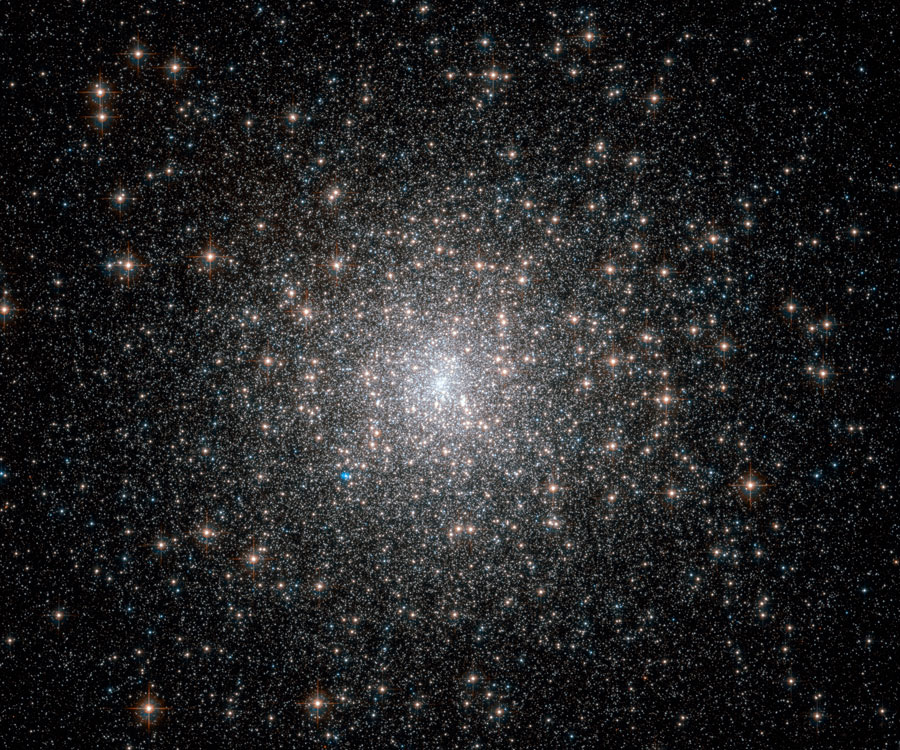
\includegraphics[width=12cm]{images/m15.jpg}
\caption[M15 Globular Cluster]{Globular Cluster M15, taken by the Hubble Space Telescope with an exposition time of 900 seconds. Image by NASA}
\end{figure}

To ensure the stability of an isolated cluster, the average speed of its individual stars must not exceed the escape velocity from the cluster. If this occurred, the stars would escape into space, and the cluster would dissipate. If the stellar velocities are low enough to satisfy this condition, then the cluster is gravitationally bound, i.e. the force of gravity is strong enough to keep the member stars from escaping.

Due to clusters moving in various orbits in the Galaxy, they are bound together with gravitational forces that are stronger than the disrupting forces exerted on it by the Galaxy or other nearby stars, and this results in an added condition for the stability of a cluster. Another factor in the stability of clusters is size-the smaller and more compact the cluster, the greater its own gravitational binding force compared with the disrupting forces, and the more chance it has to survive to old age.

Because globular clusters are highly compact systems, they are consequently very stable, and so most globular clusters will probably maintain their identity almost indefinitely.

But even these clusters lose some stars, especially if they have a slow mass. This is due to there always being a few stars in a cluster that move faster than the cluster's average speed.

When a star escapes, it carries with it energy, removing this energy from the cluster as a whole. This eventually results in the cluster developing a tightly bound core surrounded by a rarefied halo of stars-much

In the dense core of a cluster, the stars in it occasionally collide, and some of the debris eventually coalesces. Predictions indicate that this dynamical evolution could lead to the development of a large Black Hole at the cluster's center.At the same time, a few stars in the outer parts of the cluster would continue to escape. The escape rate and dynamical evolution for the rich globular clusters are so slow that the clusters can easily survive for many billions of years, remaining mostly unchanged.

Proxima Centauri, and it is 4.2 light-years, or about 1.3 parsecs. Thus, if we were able to draw a sphere around the Sun with a radius of 1.3 parsecs, it would only contain 2 stars: the Sun and Proxima Centauri. If you were to draw this same sphere in the center of the globular cluster M13, it would contain approximately 10,000 stars.

The first globular cluster discovered, but then taken for a nebula, was M22 in Sagittarius, which was probably discovered by Abraham Ihle in 1665. This discovery was followed by that of southern Omega Centauri (NGC 5139) by Edmond Halley on his 1677 journey to St. Helena. This "nebula" had been known but classified as star since ancient times. Next followed the discovery of M5 in Serpens Caput by Gottfried Kirch in 1702, and that of M13 in Hercules, again by Halley, in 1714. De Chéseaux's list of (21) nebulae of 1746 contains, in addition, two new globular clusters, M71 and M4, while Jean-Dominique Maraldi discovered M15 and M2 in September of this year (1746). Guillaume Legentil possibly or probably discovered NGC 6712 in 1749. Nicholas Louis de Lacaille's catalog of (42) southern "nebula" of 1751-52 contains 8 globular clusters (among them 5 new ones), while Messier's catalog of 110 objects contains a total of 29 globulars, 20 of them new discoveries. Charles Messier was the first to resolve one globular cluster, M4, but still referred to the other 28 of these objects in his catalog as "round nebulae." Thus, in summer 1782, before William Herschel started his comprehensive deep sky survey with large telescopes, there were 34 globular clusters known. Herschel himself discovered 36 new globulars, bringing the number of known globulars to 70. He was the first to resolve virtually all of them into stars, and coined the term "globular cluster" in the discussion adjacent to his second catalog of 1000 deepsky objects (1789).

Home/News/Hubble observations cast further doubt on how globular clusters formed
submit to reddit23Share on print
Hubble observations cast further doubt on how globular clusters formed
A theory to explain how the Milky Way’s mixed-generation globular clusters formed doesn’t work in a nearby dwarf galaxy.

New observations of the clusters show they are very similar to those found in our galaxy, the Milky Way. The finding is at odds with leading theories on how these clusters form — in these theories, globular clusters should be nestled among large quantities of old stars — and so the mystery of how these objects came to exist deepens.
NASA/ESA/S. Larsen (Radboud University, the Netherlands)
Thanks to the NASA/ESA Hubble Space Telescope, some of the most mysterious cosmic residents have just become even more puzzling. New observations of globular clusters in a small galaxy show they are very similar to those found in the Milky Way, and so must have formed in a similar way. One of the leading theories on how these clusters formed predicts that globular clusters should only be found nestled in among large quantities of old stars. But these old stars, though rife in the Milky Way, are not present in this small galaxy, and so the mystery deepens.
 
Globular clusters — large balls of stars that orbit the centers of galaxies but can lie very far from them — remain one of the biggest cosmic mysteries. They were once thought to consist of a single population of stars that all formed together. However, research has since shown that many of the Milky Way's globular clusters had far more complex formation histories and are made up of at least two distinct populations of stars.
 
Of these populations, around half the stars are a single generation of normal stars that were thought to form first, and the other half form a second generation of stars, which are polluted with different chemical elements. In particular, the polluted stars contain up to 50–100 times more nitrogen than the first generation of stars.

The proportion of polluted stars found in the Milky Way's globular clusters is much higher than astronomers expected, suggesting that a large chunk of the first-generation star population is missing. A leading explanation for this is that the clusters once contained many more stars, but a large fraction of the first-generation stars were ejected from the cluster at some time in its past.

Before now, we didn't know whether globular clusters in smaller galaxies had multiple generations or not, but our observations show clearly that they do!

This finding means that a leading theory on how these mixed-generation globular clusters formed cannot be correct, and astronomers will have to think once more about how these mysterious objects in the Milky Way and further afield came to exist.

Radial velocity measurements have revealed that most globulars are moving in highly excentric elliptical orbits that take them far outside the Milky Way; they form a halo of roughly spherical shape which is highly concentrated to the Galactic Center, but reaches out to a distance of several 100,000 light years, much more than the dimension of the Galaxy's disk. As they don't participate in the Galaxy's disk rotation, they can have high relative velocities of several 100 km/sec with respect to our solar system; this is what shows up in the radial velocity measurements. Ninkovic (1983) has estimated excentricities of globular cluster orbits.

To determine the physical orbits of globular clusters, it is required to know their proper motions in addition to the radial velocities. Cudworth and Hanson (1993) undertook some first rough determinations of proper motions with respect to background galaxies. From these and similar measurements, Van den Bergh (1995) estimated perigalactic distances, and Dauphole et.al. (1996) calculated first approximate orbits. Much more acurate data for proper motions became only available from astrometrical data obtained with ESA's Hipparcos satellite in 1997, from which space motions (Geffert et.al. 1997) and approximate orbits (Brosche et.al. 1997) could be determined.

\subsection{Basics}

\subsection{Formation and evolution}

The formation of Globular Clusters is not well understood yet, and we only hav crude ideas of their typical states right after they have reached the dynamical equilibrium.

Relaxation pretty much erases the cluster's memory of it's initial state so the results for gravitational stable systems can be reached using a wide range of initial conditions.

Since the relaxation time is inversely proportional to density evolution due to relaxation proceeds most rapidly in the dense central regions of the clusters. Within this central region that is relaxed, the distribution function $f$ and the density distribution should be approximate to a isothermal distribution, this means that the distribution function must be approximately Maxwellian at energies well bellow the escape energy. We asume that in the outer parts of the clusters the relaxation time is long and encounters have relatively little effect.

Clusters lose mass from stellar evolution: Our stellar evolution theories show us that stars often eject mass from their surfaces near the ends of their lives. For the mass-losing stars inside globular clusters, the ejected mass is likely to escape the cluster, either because the ejection velocity exceeds the escape speed from the cluster or because it interacts with the galactic gas when the cluster is passing throw the disk. So we conclude that the clusters lose mass as stars evolve. It must be mentioned that the evolution timescale of a typical population of strs is usually much longer than the crossing time in the cluster.

The mass lost by a cluster due to stellar evolution depends on the initial mass function  which specifes the distribution of masses of stars just after they have formed and the initial-final mass function. 

Now, when we talk about the evolution of the Globular Clusters, we must see how the mass distribution evolves over time. In an isolated cluster, that began as a Plummer model 

\begin{figure}[H]
\centering
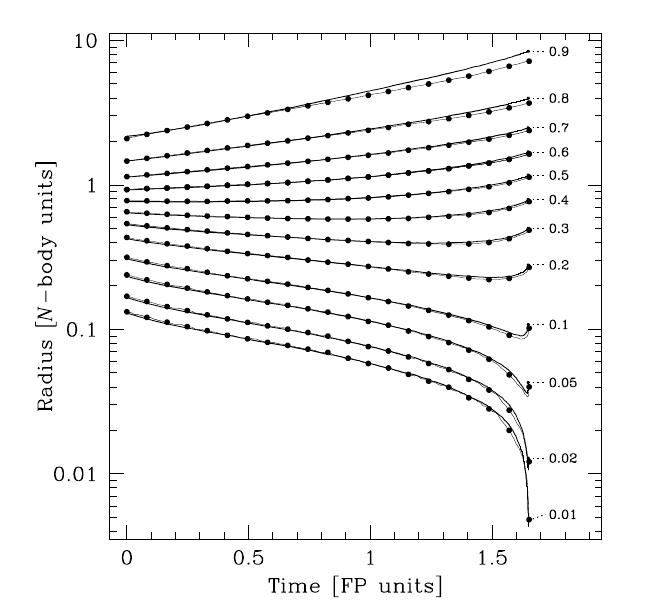
\includegraphics[width=12cm]{images/core_collapse.png}
\caption[M]{GA}
\end{figure}

Efforts are under way by several groups to produce more realistic simulations that properly include the effects
of star formation, but the existing results suggest that the first star formation may occur in gas that has become highly condensed at the centers of the first dark-matter halos to form; even though such systems may not closely resemble most present-day galaxies, they may still be of interest as the possible birth sites
of globular clusters, as will be discussed further below. The most realistic simulations of the formation of a spiral galaxy like our own have been made by Katz (1992) and Steinmetz \& Muller (1994, 1995), who have simulated the evolution of a spherical galaxy-sized piece of a standard ‘cold dark matter’ universe which is arbitrarily given the appropriate amount of angular momentum. The results show an initial chaotic stage during which mergers between clumps build up a dark halo and a stellar spheroid, followed by a period during which the remaining gas organizes itself into a disk. During the initial chaotic stage several small satellites are formed by the condensation of gas in peripheral dark-matter clumps, and these satellites may survive for a few
orbits before being disrupted and merged into the forming galaxy. It is plausible that such small satellites could be the birth sites of globular clusters, as in the hypothesis of Searle (1977) and Searle \& Zinn (1978) that the globular clusters in the outer halo of our Galaxy were formed in protogalactic ‘fragments’ which
survived for a time as independent star-forming systems before being merged to build up the halo

In several earlier reviews of globular cluster chronology, it was concluded that the globular clusters in our Galaxy are not all coeval and that age differences of several Gyr exist in at least a few well-studied cases (e.g., Larson 1990a, 1992b). This conclusion still appears to be valid, and it is supported by the most recent discussion of this subject by Chaboyer, Demarque, \& Sarajedini (1996), which is based on new age estimates for 43 globular clusters


 Although our Galaxy has evidently not experienced any further major accretion events capable of disrupting the disk, it is possible that minor accretion events affecting only the halo and not the disk have continued to occur (Navarro, Frenk, \& White 1994); indeed, several contributors to this meeting have already noted that our Galaxy is apparently just now accreting the recently discovered Sagittarius dwarf galaxy, which contains four already known outer-halo globular clusters including Arp 2 and Ter 7 

Most of the clusters
whose masses are larger than 105 M have lifetimes longer than the Hubble tim

An important recent advance in our understanding of star formation has
been the realization that nearly all stars are formed in groups or clusters of
some kind. Even in the nearby Taurus-Auriga region, which has been regarded
as prototypical of isolated star formation, the T-Tauri stars are actually mostly
distributed in a hierarchy of small groups of various sizes

\subsection{Observational Properties}

The HR diagram for a typical globular cluster looks very different than that of an open cluster. There are no Main Sequence stars of types OBAF, but there are many red giants. The brightest stars in a globular cluster are those at the tip of the red giant branch in the HR diagram, which explains the red appearance of the bright stars in color images of the clusters. You can also see stars populating the horizontal branch (and also why it is called the horizontal branch), the asymptotic giant branch, and even some stars that have colors and magnitudes of F stars, but far fewer than the G stars just below and to the right of them on the Main Sequence.

\begin{figure}[H]
\centering
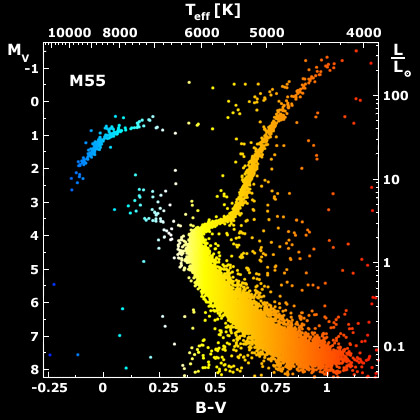
\includegraphics[width=10cm]{images/m55_diagram.jpg}
\caption{Color Magnitude diagram of M55. Image by NASA}
\end{figure}

(incluir poblaciones estelares)

\section{Stellar System Dynamics}

\subsection{Potential Theory of Spherical Systems}

(we focus on globular clusters)

The velocity dispersion profile of bright stars flattens when dark matter is present.

\subsection{Colisionless Systems}

\begin{equation}
\dfrac{df}{dt}=0
\end{equation}

\subsection{Dynamics}

(Collisionless Boltzmann equation, Distribution Function, Jeans equations)

\begin{equation}
\frac{df}{dt}=0
\end{equation}

\begin{equation}
\frac{\partial f}{\partial t}+\sum_{i=1}^{3}\frac{\partial f}{\partial x_{i}}\dot{x_{i}}+\sum_{i=1}^{3}\frac{\partial f}{\partial v_{i}}\dot{v_{i}}=0
\end{equation}


\begin{equation}
\dot{v_{i}}=-\frac{\partial\phi}{\partial x_{i}}
\end{equation}

\begin{equation}
\frac{\partial f}{\partial t}+\nabla f\cdot\vec{v}+\frac{\partial f}{\partial\overrightarrow{v}}\cdot\nabla\phi=0
\end{equation}

Moment of order $j$ of the distribution $f$

\begin{equation}
\overline{x^{j}}=\frac{\int x^{j}fdx}{fdx}
\end{equation}

velocity dispersion tensor:

\begin{equation}
\sigma_{ij}^{2}=\overline{v_{i}v_{j}}-\overline{v_{i}}\:\overline{v_{j}}
\end{equation}

Anysotropy parameter:

\begin{equation}
\beta=1-\frac{\left(\sigma_{\theta}^{2}+\sigma_{\phi}^{2}\right)}{2\sigma_{r}^{2}}
\end{equation}

When $\beta=1$ total anisotropy

\section{Scenario and Observations}

there is  widesprea belief that globular clusters cannot contain large amounts of dark matter, because of the Virial Theorem. This theorem relates the velocity dispersion $ \sigma $ at the center of the cluster to the total mass $M_{t}$ and to the half-mass radius $r_{h}$ of the system. For a one component globular cluster, that relation may be expresed as:

\begin{equation}
\left\langle \sigma^{2}\right\rangle \approx0.4\frac{GM_{t}}{r_{h}}
\end{equation}

However, if a dark component is also present, in the form of low-mass objects for example, the virial theorem must be modified to:

\begin{equation}
\sum_{i}M_{t}(i)\left\langle \sigma^{2}\right\rangle _{i}=E_{p}
\end{equation}

where the index $i$ refers to the different stellar species, and $E_{p}$ is the potential energy of the cluster.

\section{Simulations}

(N-body simulations, plummer sphere)